\section{Usage}
The GeoLog was designed for field scientist or anyone how is interested in monitoring the enviroment. In the development of the GeoLog it was taken into account the system would be able to perform in rough environment and could be left outside in rugged terrain.\\
The knowledge one needs for building and maintain his own GeoLog is a background in software C, C++ and knowledge in electric circuits. % %For further development one would...

\subsection{Installation}
When preparing the system for first use setup of necessary software is needed to be able to configure the sampling rate of the desired data. The user needs to be able to modify the Arduino sketch but should not be required to modify the Wixel software. Thus set up of the Arduino development enviroment is needed but for the Wixel it is optional.\\
All the required code for this system can be found under~\url{https://github.com/sveinnel/geolog}. The link~\url{https://github.com/sveinnel/geolog} will be referred as geolog-folder from here on.\\

\begin{enumerate}
\item Install the software
	\begin{enumerate}
	\item For the Arduino:
		\begin{enumerate}
		\item Start a web browser
		\item Go to~\url{http://arduino.cc/en/main/software}
		\item Install the appropriate version of Arduino IDE for your platform.
		\end{enumerate}
	\item For the Wixel:
		\begin{enumerate}
		\item Start a web browser
		\item Go to~\url{http://www.pololu.com/docs/0J46}
		\item Install the Wixel IDE, see part 3 in Pololu user's guide
		\item Follow the instructions listed in part 10.a, 10.b and 10.c, for setting up the development enviroment
		\end{enumerate}
	\end{enumerate}
\item Set up the hardware
	\begin{enumerate}
	\item Connect the components for the mother hub:
		\begin{enumerate}
		\item Follow the schematic in figure~\ref{fig:motherhub_schematic}
		\item Position the mother hub in its box as in figure~\ref{fig:Main_Open}
		\end{enumerate}
	\item Connect the components for the wireless sensor module/modules:
		\begin{enumerate}
		\item Follow the schematic in figure~\ref{fig:sensormodule_schematic}
		\item Position the components in its box as in figure~\ref{fig:Wixel_sensor}
		\end{enumerate}
	\end{enumerate}
\item Upload the code
	\begin{enumerate}
	\item For the mother hub:
		\begin{enumerate}
		\item Upload the application wireless\_serial.wxl on the Wixel. The application can be found under geolog-folder/Wixel/Receiver
		\item Upload the script MainRunner.ino on the Arduino. The script can be found under geolog-folder/Software
		\end{enumerate}
	\item For the wireless sensor module/modules:
		\begin{enumerate}
		\item Upload the application wireless\_serial.wxl on the Wixel. The application can be found under geolog-folder/Wixel/Transmitter
		\end{enumerate} 
	\end{enumerate}
\item Place the batteries in each module:
	\begin{enumerate}
	\item The mother hub needs a power source of 5-9V
	\item The wireless sensor modules need a power source of 2.7-6.5V
	\end{enumerate}
% TODO:
%\item Check if the device is correctly setup
%	\begin{enumerate}
%	\item Each of the Wixels should be blinking the green led with the frequency 1Hz
%	\item If the red led is constantly on the Wixel is not finding the correct way for communicating
%	\end{enumerate}
\end{enumerate}
Set the sampling frequency and the data transmission time for the GeoLog to the desired values. To set the values the MainRunner.ino sketch needs to be modified. The sketch can be found under geolog-folder/Software. Change the defined constants SAMPLE\_DATA\_FREQ and SEND\_DATA\_FREQ in line 13 and 14, the values for the sampling time should be given in milliseconds. Then compile the modified MainRunner.ino sketch on the Arduino then the GeoLog should be ready for collecting data. %If there is something the did not go as planed check the instructions for error procedure
\begin{figure}[H]
\centering
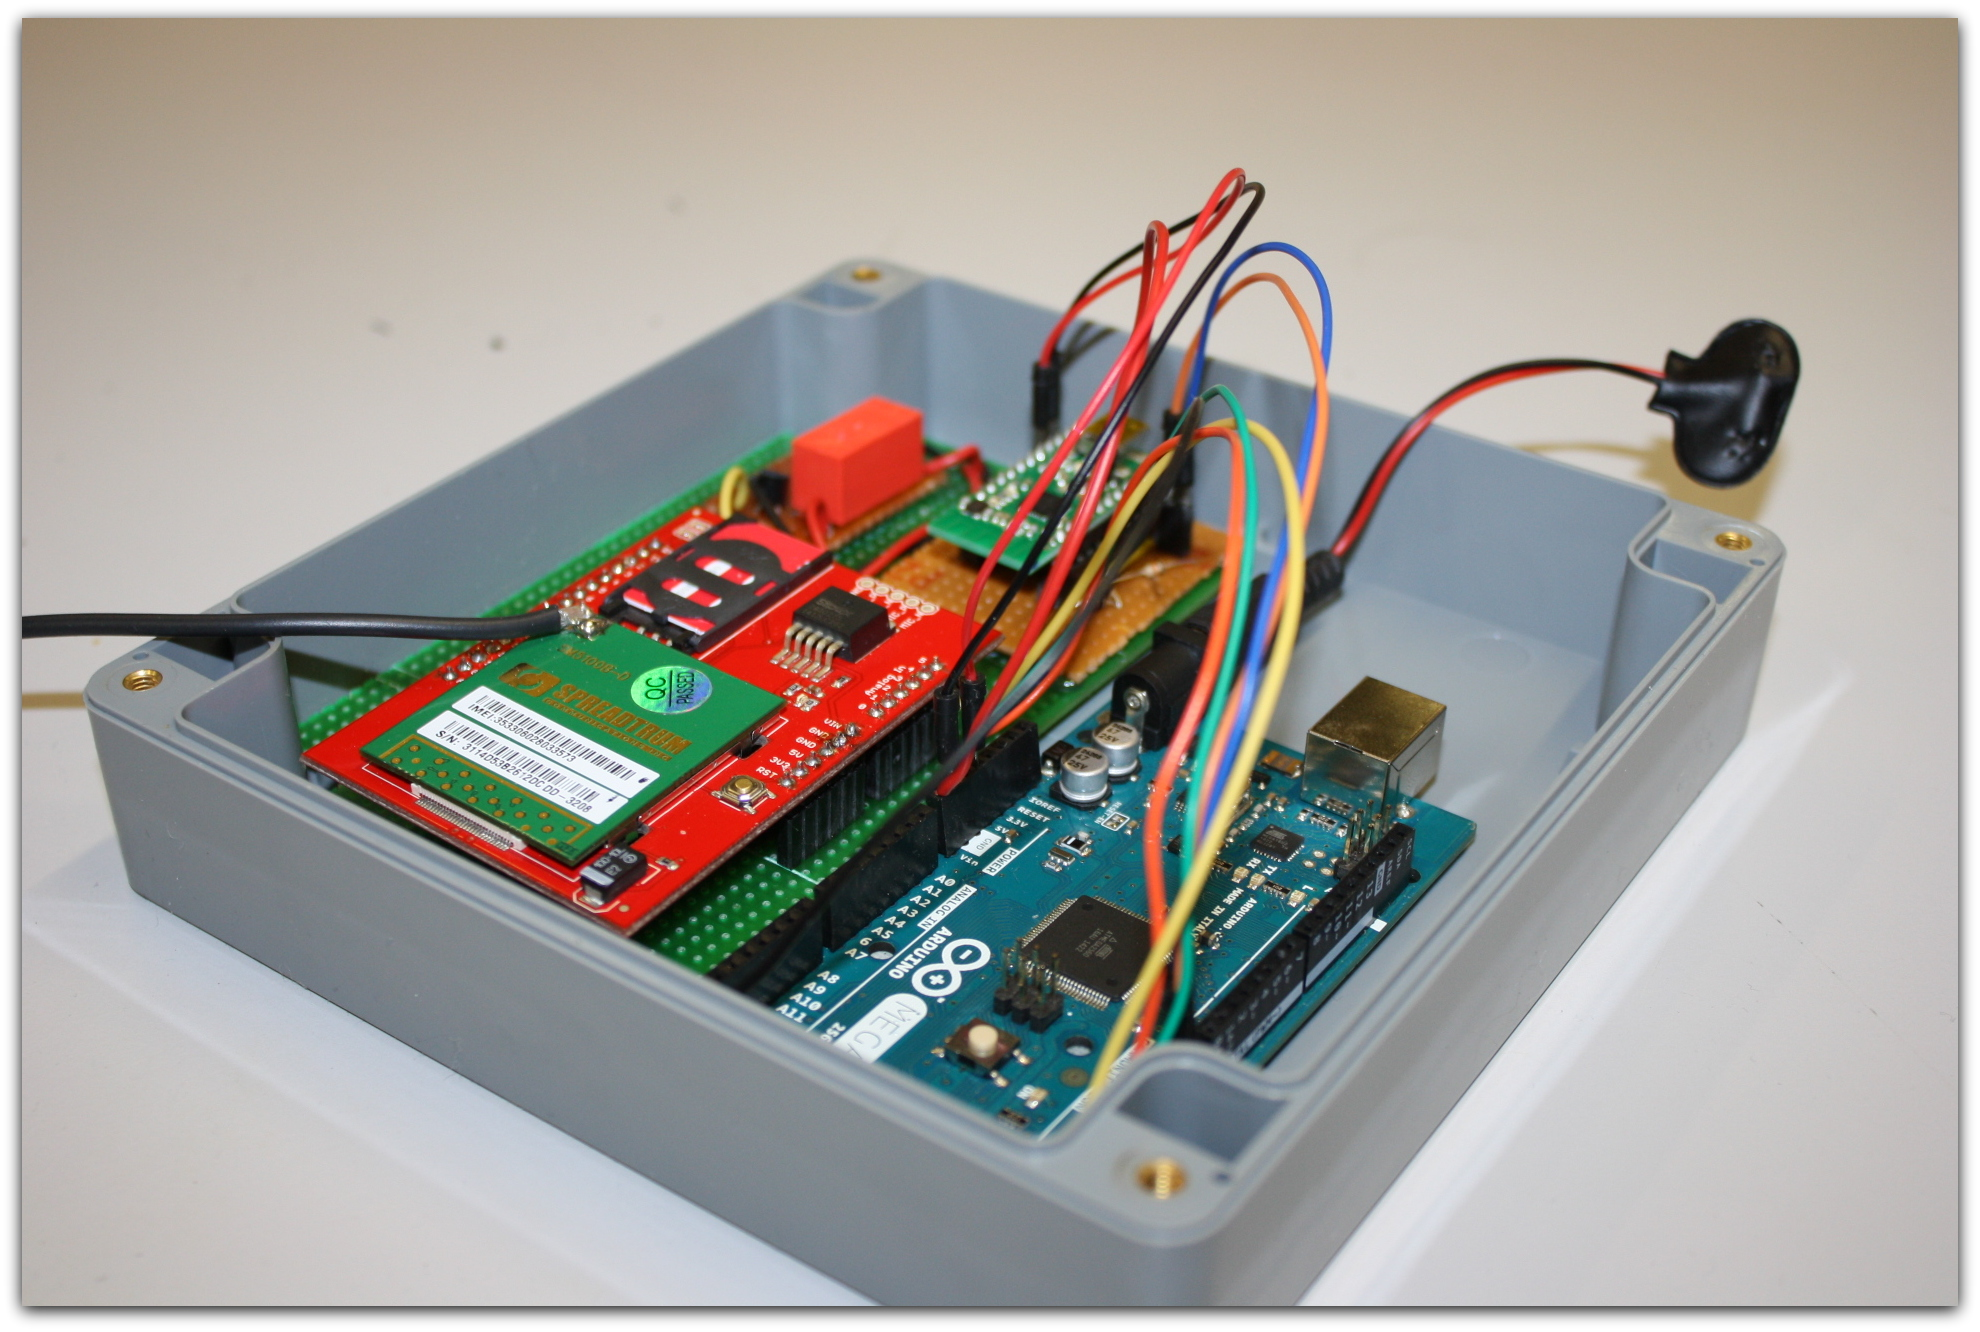
\includegraphics[width=0.6\linewidth]{graphics/Main_Open.jpg}
\caption{The mother hub displayed in its box\label{fig:Main_Open}}
\end{figure}
\begin{figure}[H]
\centering
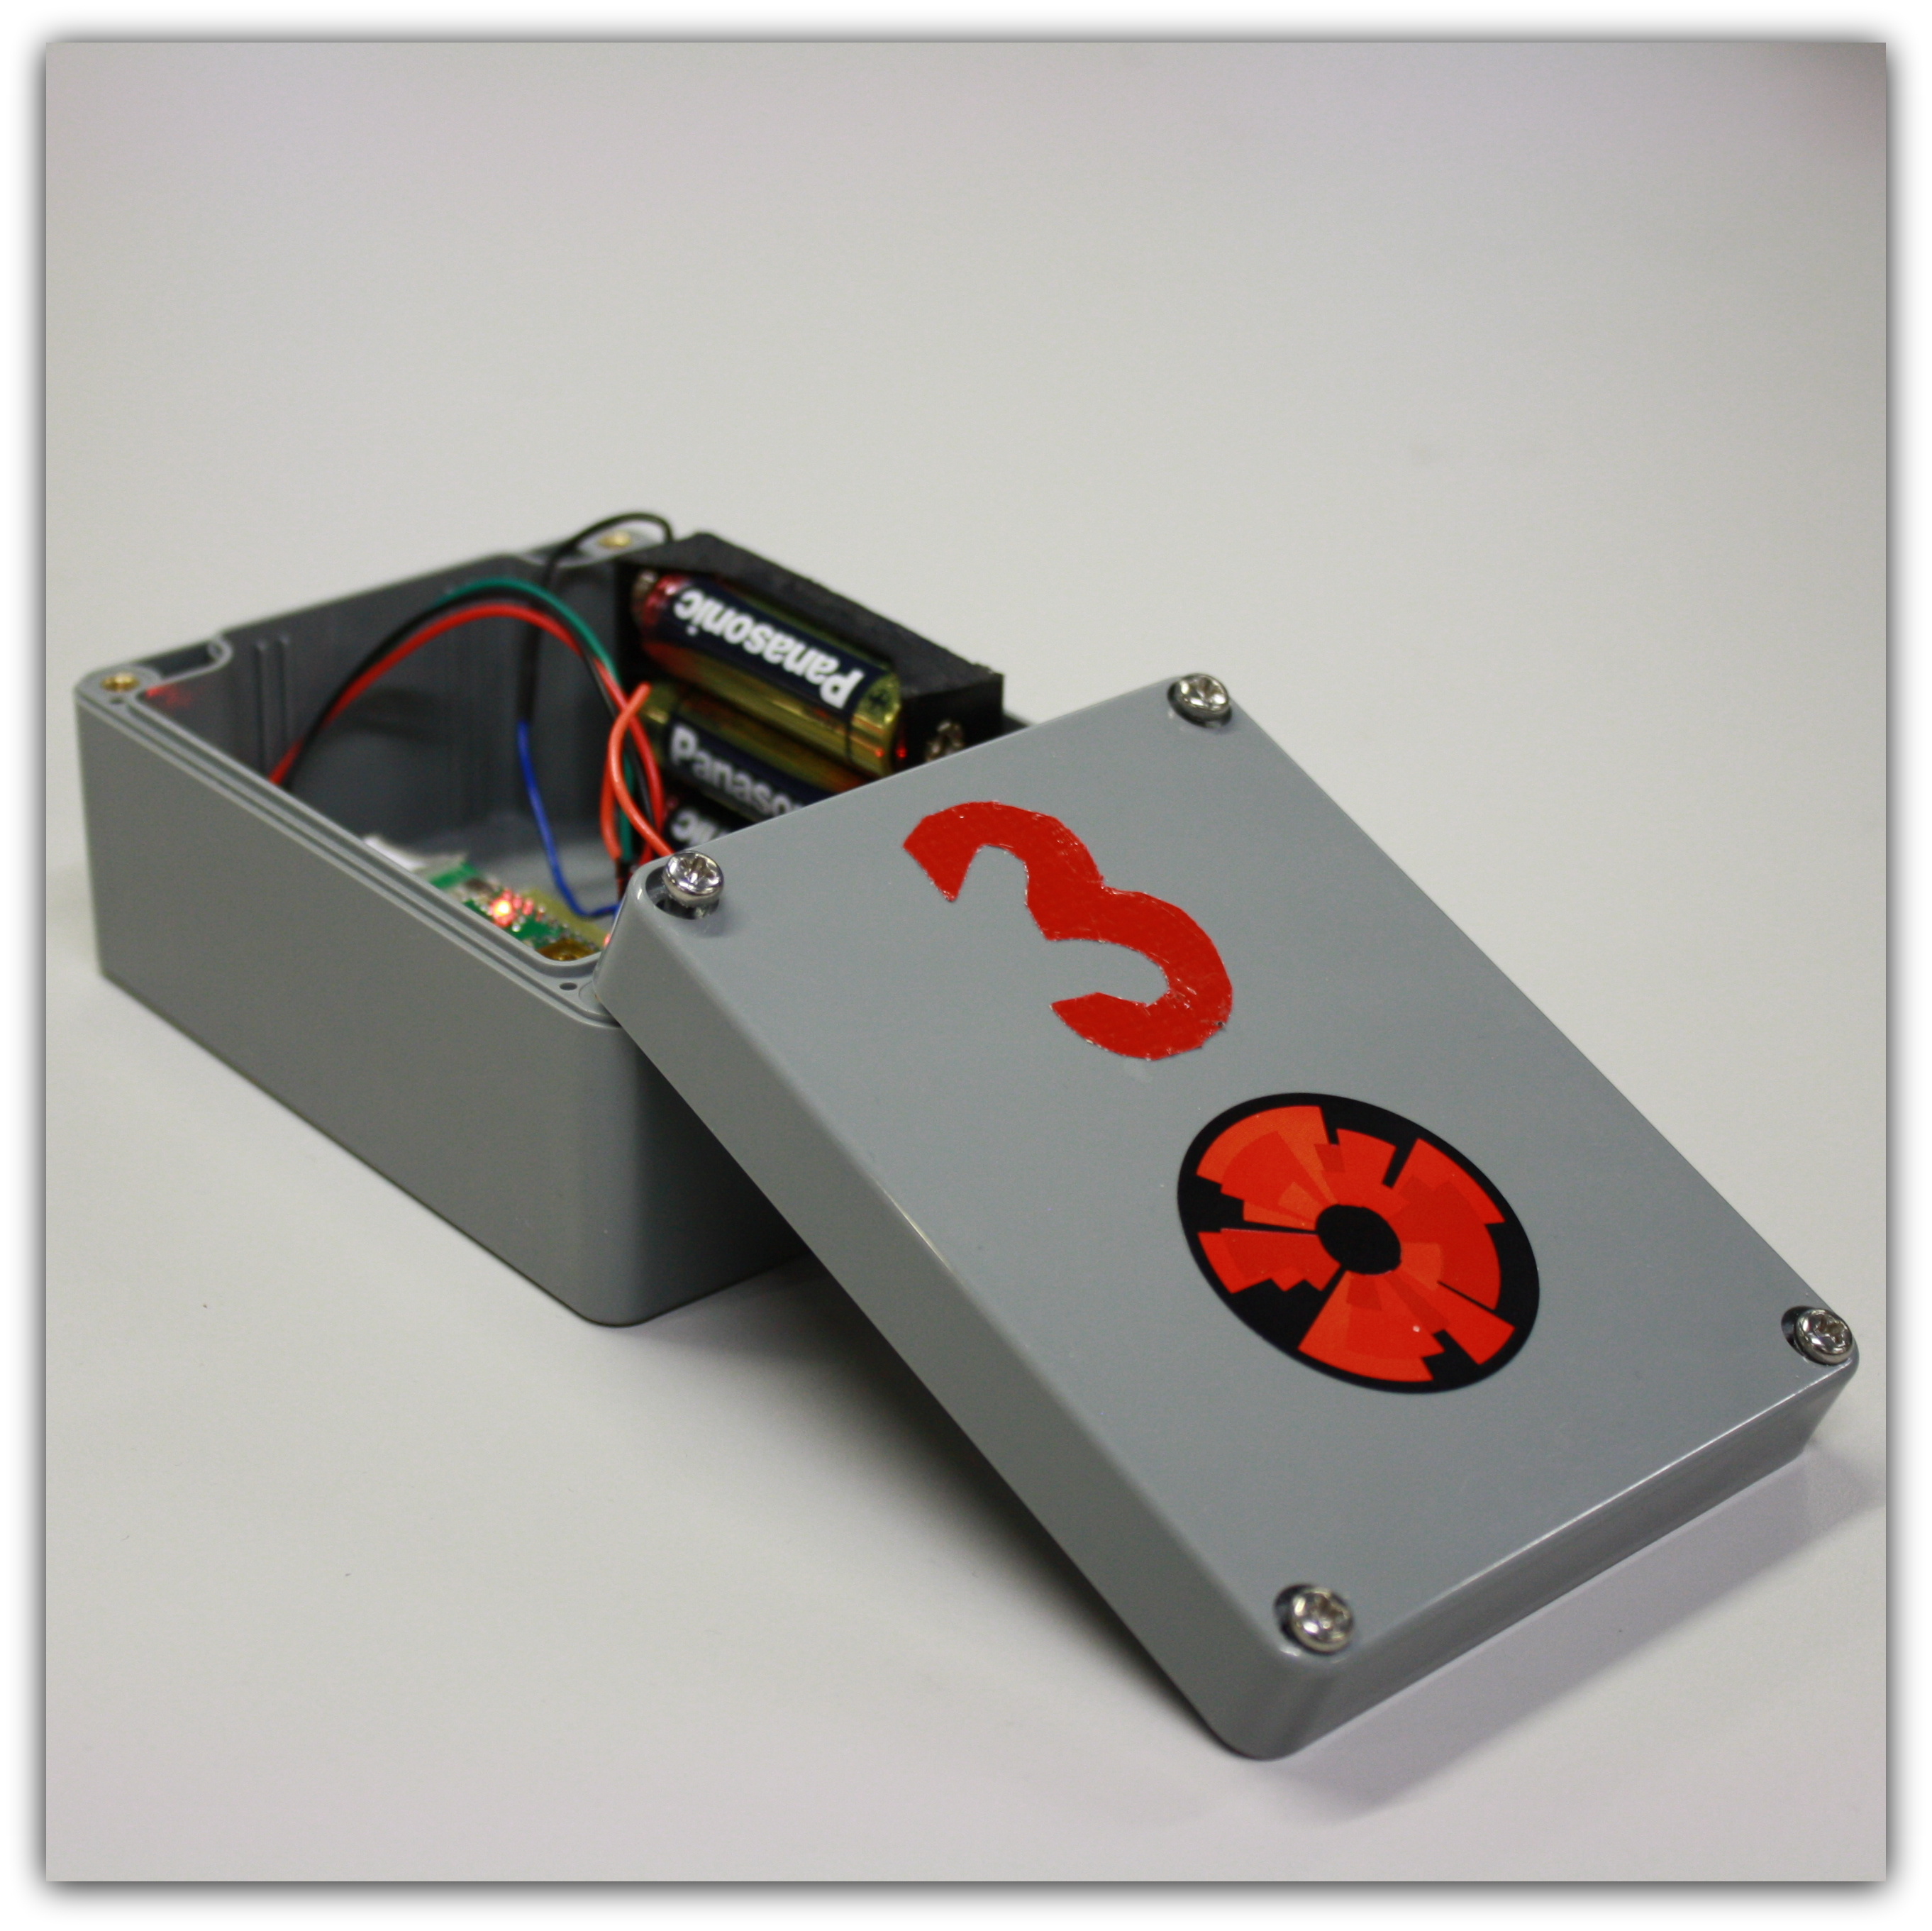
\includegraphics[width=0.6\linewidth]{graphics/Wixel_sensor.jpg}
\caption{The wireless sensor module in its box\label{fig:Wixel_sensor}}
\end{figure}
To prep the GeoLog for transport the batteries need to be removed out of the box for each module. The boxes should be securely closed with the four screws in each corner. Then the GeoLog is ready for travel.\\
To unpack the GeoLog open the boxes, insert the batteries and securely close the boxes again.\\
\textbf{Warning: If the boxes are not closed securely, they might start leaking. That could damage the electronics}.

\subsection{Instructions}
Once the system is setup the user should be able to position the GeoLog in the site where data will be collected. Spread out the wireless sensor modules around the mother hub, such they can sample the desired data.\\
\textbf{Warning: the Wixel sensor module can not be placed more than 15 meters away from the mother hub}. The Wixels will not be able to transmit the data over a distance of more than 15 meters in clear line of sight.\\
If everything has been setup correctly the raw data will be transmitted over to the HTTP server.\\
Extra preparation or calibration should not be needed. The only routine maintenance needed is replacement of battery packs when the ones installed run out.\\\\ % TODO: check if there is need for more precise definition of runing out of battery...
If the GeoLog is not transmitting the data over to the server the user can manually request a transmission to be sent. In order to request a transmission the user needs to connect a wire from pin 51 on the Arduino to the ground see figure~\ref{fig:userPins}. The red light on the GSM module should turn on for a short while (10 to 30 seconds) and turn off again. If the data does not arrive on the HTTP server the user might be forced to clear the EEPROM on the Arduino and try again. To clear the EEPROM the user needs to connect a wire from pin 50 on the Arduino to the ground, see figure~\ref{fig:userPins}. The led at pin 13 on the Arduino board will be turned on until the EEPROM has been fully cleared. Once the EEPROM has been cleared the user should attempt once again to manually request a transmission of data to the HTTP server. If the data does still not arrive on the HTTP server the user is advised to go over the installation process once more to ensure everything is correctly connected and is operating the correct software on each module.

\begin{figure}[H]
\centering
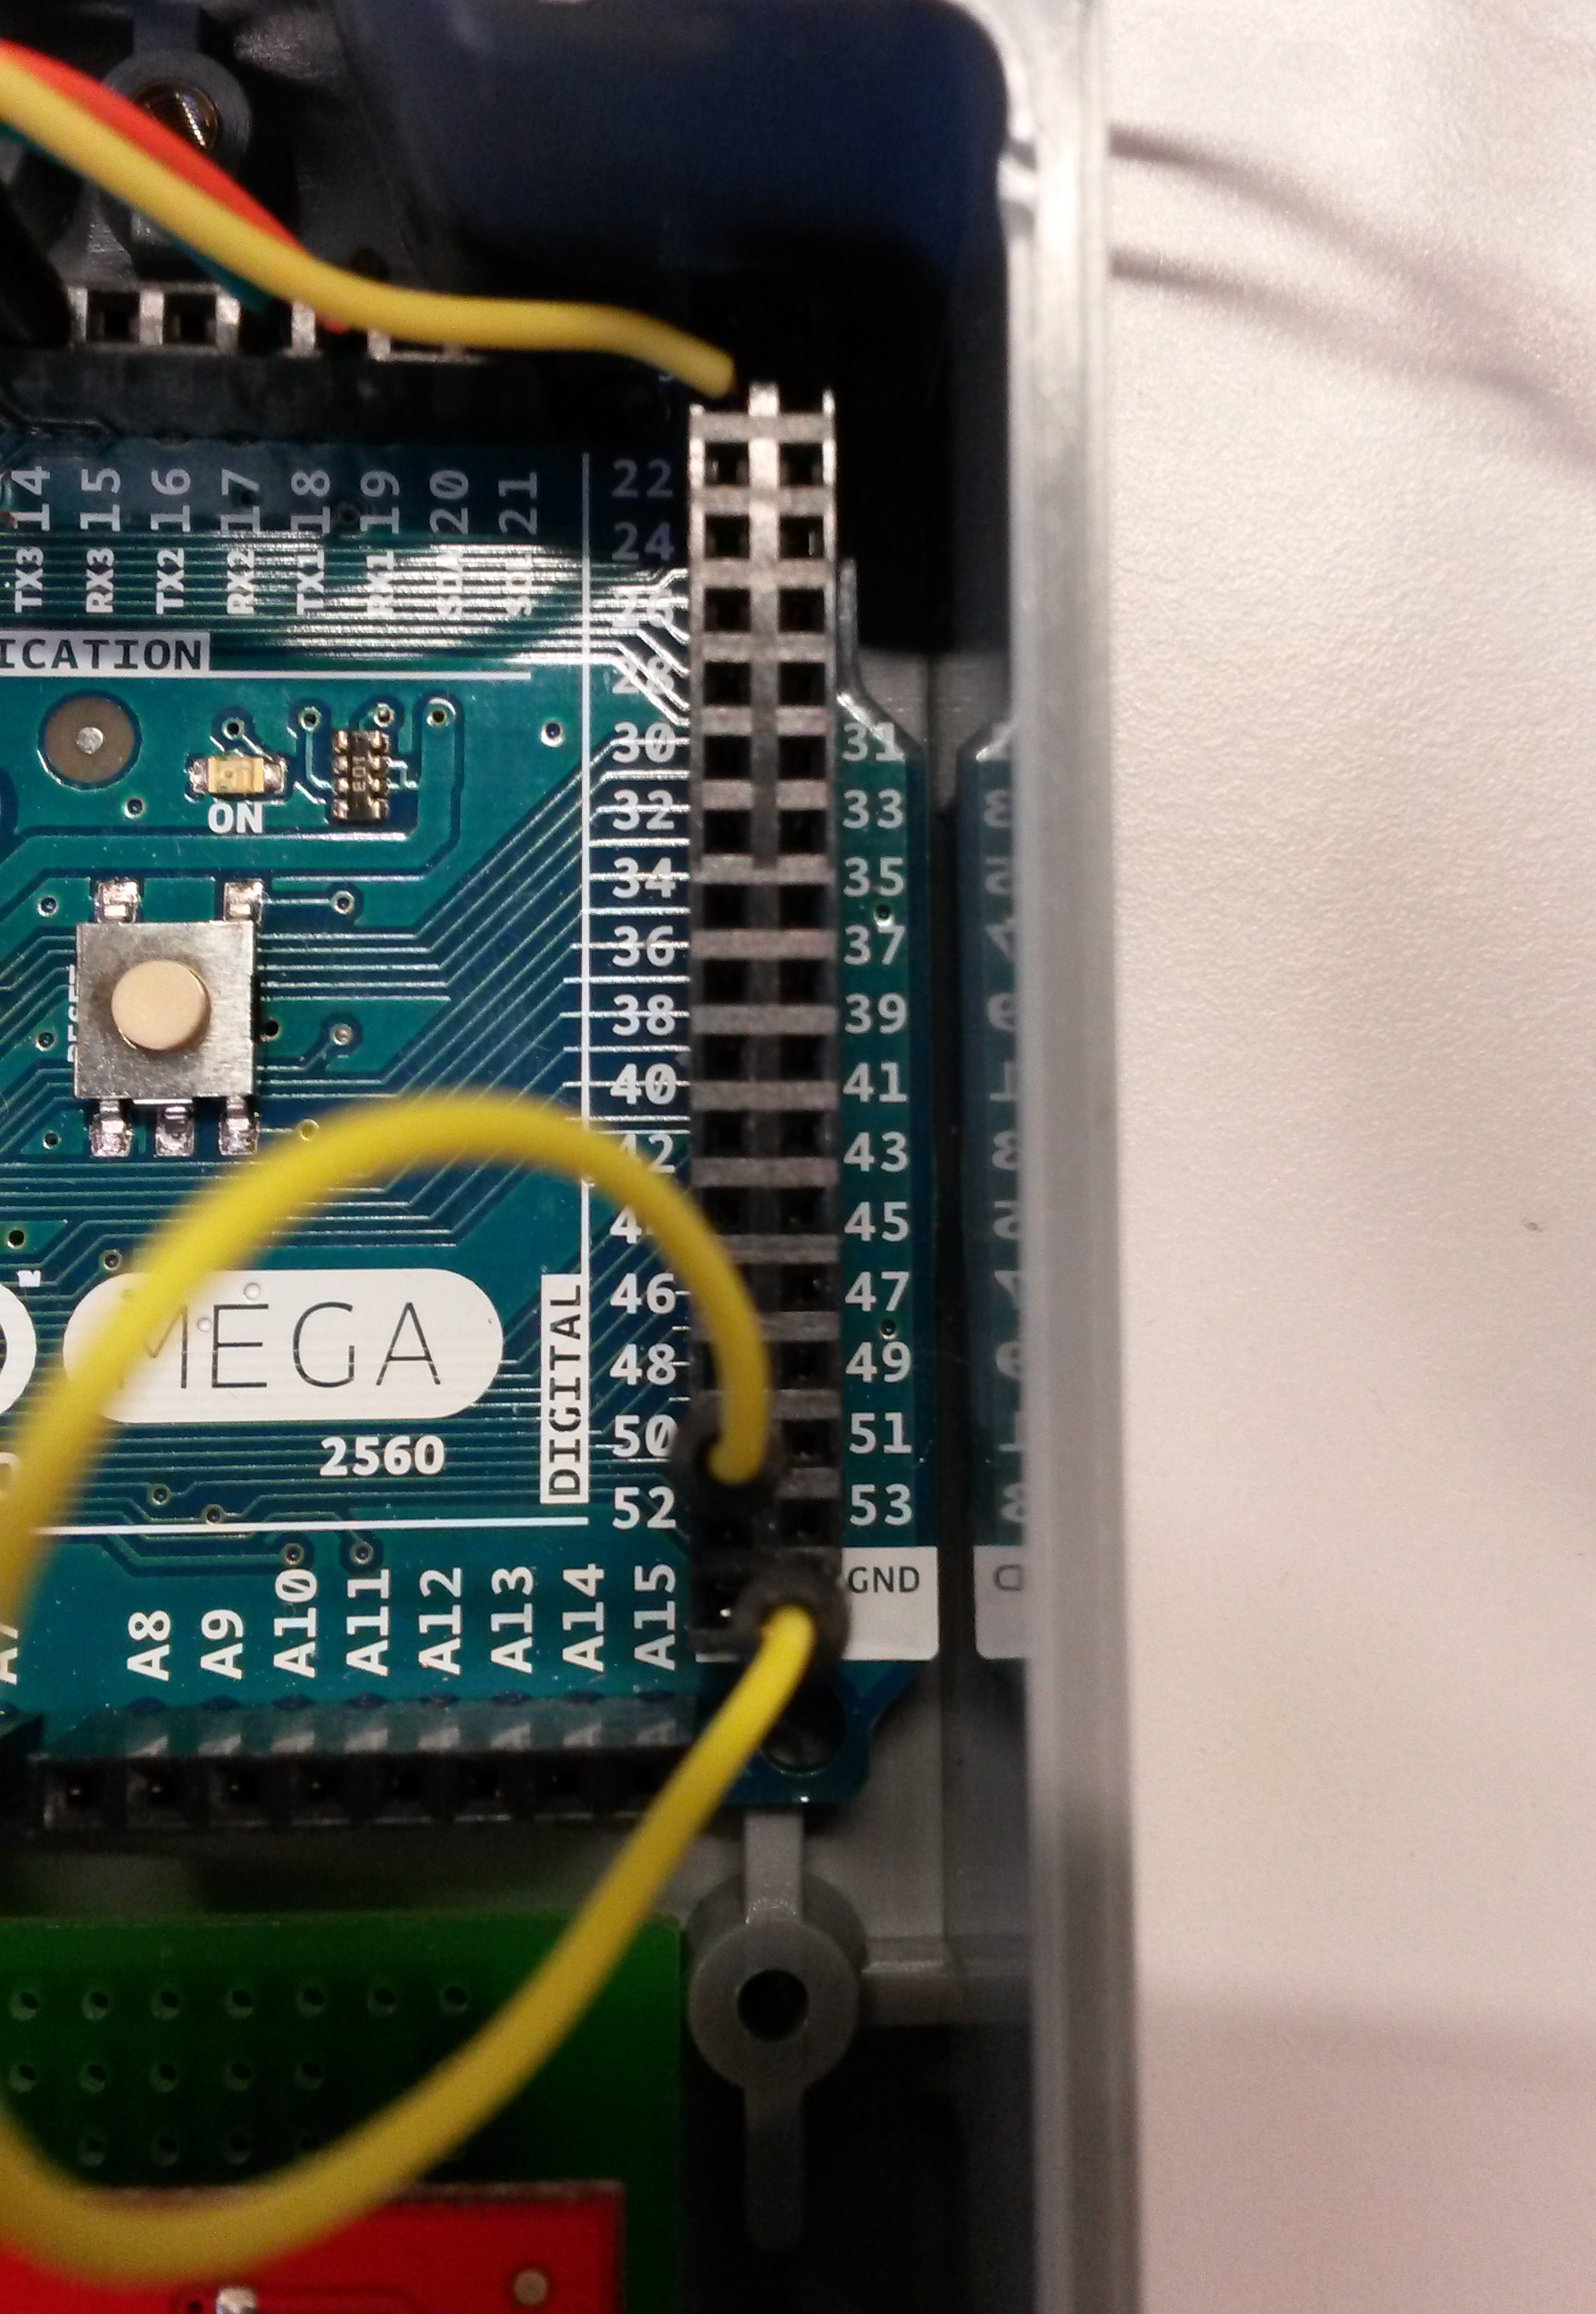
\includegraphics[width=0.6\linewidth]{graphics/userPins.jpg}
\caption{The request transmission pin 51 and clear EEPROM pin 50 shown\label{fig:userPins}}
\end{figure}









